\chapter{TINJAUAN PUSTAKA DAN LANDASAN TEORI}


\section{Tinjauan Pustaka}
	Tinjauan pustaka dituliskan berdasar apa yang sudah Anda pelajari dalam rangka penelitian tesis S2. Susunlah tinjauah pustaka dari yang bersifat umum menuju khusus (general to specific). Tinjauan pustaka ini dipelajari dari paper-paper seminar maupun jurnal.
	
\section{Landasan Teori}
	Landasan teori dituliskan berdasar tinjauan pustaka, sebagai bentuk yang lebih spesifik sesuai dengan arah penelitian Anda. Landasan teori ini didapat dari paper maupun buku, yang mendasari metodologi penelitian yang dibahas di Bab III.


\subsection{Penggunaan Sitasi}
Contoh penggunaan sitasi \cite{lukito2016,santosa2011user}
\cite{setiawan2014fuzzy} \cite{wibowo2014line} \cite{marenda2016digitory} \cite{wibirama2013dual,wibowo2016clustering}

\subsection{Penulisan Gambar}

\begin{figure}[h]
	\centering
	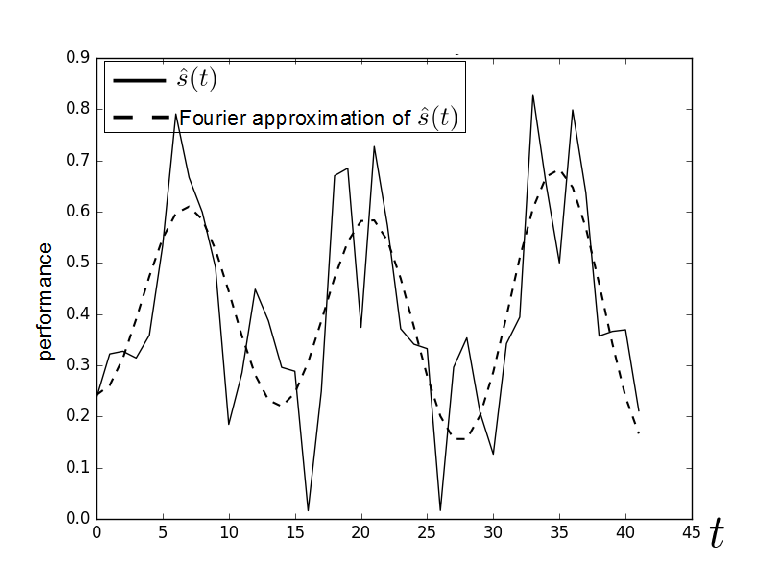
\includegraphics[width=10cm]{contents/chapter-2/sample-fig.png}
	\caption{Contoh gambar.}
	\label{Fig: Contoh gambar}
\end{figure}

Contoh gambar terlihat pada Gambar \ref{Fig: Contoh gambar}. Gambar diambil dari \cite{wibowo2016clustering}.

\subsection{Penulisan Tabel}
\begin{table}[h]
	\caption{tabel ini}
	\vspace{0.5em}
	\centering
	\begin{tabular}{|c|c|c|}
		\hline
		ID & Tinggi Badan (cm) & Berat Badan (kg) \\
		\hline \hline
		A23 & 173 & 62 \\
		A25 & 185 & 78 \\
		A10 & 162 & 70 \\ \hline
	\end{tabular}
	\label{Tab: Tabel Tinggi Berat}
\end{table}
Contoh penulisan tabel bisa dilihat pada Tabel \ref{Tab: Tabel Tinggi Berat}.

\subsection{Penulisan formula}
Contoh penulisan formula
\begin{equation}
L_{\psi_z} = \{ t_i \mid v_z(t_i) \le \psi_z \}
\end{equation}

Contoh penulisan secara \textit{inline}: $L_{\psi_z} = \{ t_i \mid v_z(t_i) \le \psi_z \}$.